% !TeX TS-program = xelatex
% !BIB TS-program = bibtex

% Full instructions available at:
% https://github.com/pcafrica/focus-beamertheme


\documentclass{beamer}
\usepackage{blindtext} %This package generates automatic text
\usepackage{epigraph}
\usepackage{tikz}
\usetikzlibrary{arrows.meta, positioning}
\usetheme{focus}


\definecolor{main}{RGB}{142, 111, 62}
% \definecolor{text}{RGB}{60, 60, 80}
% \definecolor{background}{RGB}{255, 255, 255}

\title{An Effect System for Algebraic Effects \& Handlers}
% \subtitle{Subtitle}
\author{Asha}
\titlegraphic{\epigraph{Programming Languages are like saddles, We don't make the saddle for the horse, The horse doesn't need the saddle, It does not want it}{\textit{Andrej Bauer \\ OPLSS 2018}}}

% \titlegraphic{\includegraphics[scale=1.25]{focus-logo.pdf}}
% \institute{Institute Name \\ Institute Address}
\date{\today}

% Footline info is printed only if [numbering=fullbar].
%\footlineinfo{Custom footline text}

\begin{document}
    \input{beginning}
    
    % Use starred version (e.g. \section*{Section name})
    % to disable (sub)section page.
    
    % \input{tt}
    \section{Introductions}
\subsection{Algebraic Effects \& Handlers}


\begin{frame}{The Problem with Traditional Type Systems}
  \begin{itemize}
    \item Traditional type systems describe \textbf{entities of pure computation}, but not \textbf{computational effects}.
    \vspace{0.5em}
    \item Effects (like exceptions, I/O, state) are:
      \begin{itemize}
        \item Invisible to the type system
        \item Difficult to reason about or restrict
        \item Cause code to be less modular and harder to verify
      \end{itemize}
    \vspace{0.5em}
    \item There is a need to unify the formal definition of computational effects under some abstract definition.
  \end{itemize}
\end{frame}
\begin{frame}{What Are Algebraic Effects?}
  \begin{itemize}
    \item \textbf{Algebraic effects} describe computational effects via \textit{abstract operations}.
    \vspace{0.5em}
    \item Examples:
      \begin{itemize}
        \item \texttt{raise : string $\to$ $\_$} \hfill (exceptions)
        \item \texttt{get : unit $\to$ int} \hfill (state)
        \item \texttt{choose : unit $\to$ bool} \hfill (nondeterminism)
      \end{itemize}
    \vspace{0.5em}
    \item Think of them as \textbf{requests} for effects, not implementations.
    \vspace{0.5em}
    \item Separate the notion of \textit{what an effect is} from \textit{how it is handled}.
  \end{itemize}
\end{frame}
% \begin{frame}{What Are Algebraic Effects?}
% \centering
% 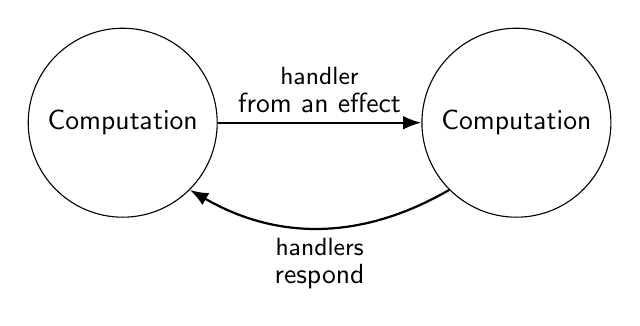
\begin{tikzpicture}[
    every node/.style={font=\sffamily},
    computation/.style={draw, circle, minimum size=2.4cm, align=center},
    >=Latex
]

% Nodes
\node[computation] (C1) at (0, 0) {Computation};
\node[computation] (C2) at (5, 0) {Computation};

% Arrows
\draw[->, thick] (C1.east) -- node[above, align=center] {\small handler\\[-2pt]from an effect} (C2.west);
\draw[<-, thick] (C1.south east) to[bend right=30] node[below, align=center] {\small handlers\\[-2pt]respond} (C2.south west);

\end{tikzpicture}
% \end{frame}

\begin{frame}{Handlers: The Dual Viewpoint}
  \begin{columns}[c]
    \column{0.55\textwidth}
    \begin{itemize}
      \item \textbf{Handlers} define how effects are interpreted.
      \vspace{0.5em}
      \item Think of them as \textbf{responders} to abstract operations.
      \vspace{0.5em}
      \item Example clauses:
      \begin{itemize}
        \item \texttt{val x $\Rightarrow$ c\textsubscript{val}}
        \item \texttt{op y k $\Rightarrow$ c\textsubscript{op}}
      \end{itemize}
      \vspace{0.5em}
      \item First-class and composable.
    \end{itemize}

    \column{0.45\textwidth}
    \centering
    % \includegraphics[width=0.9\textwidth]{computation_handler_diagram.png}
    \resizebox{0.8\linewidth}{!}{%
  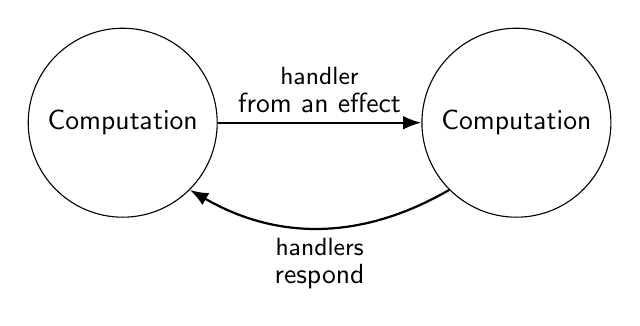
\begin{tikzpicture}[
    every node/.style={font=\sffamily},
    computation/.style={draw, circle, minimum size=2.4cm, align=center},
    >=Latex
]

% Nodes
\node[computation] (C1) at (0, 0) {Computation};
\node[computation] (C2) at (5, 0) {Computation};

% Arrows
\draw[->, thick] (C1.east) -- node[above, align=center] {\small handler\\[-2pt]from an effect} (C2.west);
\draw[<-, thick] (C1.south east) to[bend right=30] node[below, align=center] {\small handlers\\[-2pt]respond} (C2.south west);

\end{tikzpicture}
}
    
  \end{columns}
\end{frame}

\begin{frame}[fragile]{Motivation Through Examples}
\vspace{-0.5em}
\begin{block}{Nondeterministic Choice with \texttt{Choose}}
\begin{verbatim}
effect Choose : unit -> bool

let flip = Choose()

with handler
  val x => x
  | Choose() k => k(true) || k(false)
handle
  if flip then "Heads" else "Tails"
\end{verbatim}
\end{block}
\vspace{0.5em}
\begin{itemize}
  \item \texttt{Choose()} is an effect request — “flip a coin”
  \item Handler responds by exploring \texttt{true} and \texttt{false}
  \item Result: evaluates to both “Heads” and “Tails”
\end{itemize}
\end{frame}

\begin{frame}[fragile]{Message Passing: \texttt{Send} and \texttt{Receive} Effects}
\vspace{-0.5em}
\begin{block}{\scriptsize Effect Declarations and \texttt{ping}}
\begin{scriptsize}
\begin{verbatim}
effect Send : int -> unit
effect Receive : unit -> int

let ping =
  for i = 1 to 3 do
    Send(i);
    let msg = Receive() in
    Printf.printf "Ping received %d\n" msg
  done
\end{verbatim}
\end{scriptsize}
\end{block}
\vspace{0.3em}
\begin{itemize}
  \item \texttt{Send} and \texttt{Receive} are abstract operations.
  \item \texttt{ping} sends values and receives replies.
  \item Handler decides what message passing means.
\end{itemize}
\end{frame}
\begin{frame}[fragile]{Message Passing: The \texttt{pong} Side}
\vspace{-0.5em}
\begin{block}{\scriptsize \texttt{pong} Responds to \texttt{ping}}
\begin{scriptsize}
\begin{verbatim}
let pong =
  for _ = 1 to 3 do
    let msg = Receive() in
    Printf.printf "Pong received %d\n" msg;
    Send(msg + 100)
  done
\end{verbatim}
\end{scriptsize}
\end{block}
\vspace{0.3em}
\begin{itemize}
  \item \texttt{pong} waits for a message, processes it, and replies.
  \item Sends back \texttt{msg + 100} after each receive.
  \item This effectful back-and-forth models structured concurrency.
\end{itemize}
\end{frame}

\begin{frame}[fragile]{Message Passing via Effects: Part 3}
\vspace{-0.5em}
\begin{block}{\scriptsize The \texttt{run} Function Coordinates Both}
\begin{scriptsize}
\begin{verbatim}
let rec run pingside pongside =
  match pingside () with
  | v -> v
  | effect (Send x) k1 ->
    match pongside () with
    | v -> v
    | effect Receive k2 ->
      run (fun () -> continue k1 ()) (fun () -> continue k2 x)
  | _ -> failwith "Unexpected effect"
\end{verbatim}
\end{scriptsize}
\end{block}

\begin{itemize}
  \item Handles \texttt{Send} from \texttt{ping}, \texttt{Receive} from \texttt{pong}.
  \item Resumes each with continuation-passed values.
  \item Models **cooperative message passing** purely via effects.
\end{itemize}
\end{frame}
\begin{frame}[fragile]{6a: Programs Stay Pure, Effects Are Handled}
\vspace{-0.5em}
\begin{block}{\scriptsize Define Effects and Suspension State}
\begin{scriptsize}
\begin{verbatim}
effect Send : int -> unit
effect Receive : unit -> int

type state =
  | Done
  | Paused of int * continuation
  | PausedR of continuation
\end{verbatim}
\end{scriptsize}
\end{block}

\begin{itemize}
  \item Programs use effects via \texttt{perform}.
  \item They don’t define what sending/receiving means.
  \item Interpretation is delegated to the handler.
\end{itemize}
\end{frame}
\begin{frame}[fragile]{6b: Programs as Pure Computations}
\vspace{-0.5em}
\begin{block}{\scriptsize Handlers Manage Interaction, Not the Programs}
\begin{scriptsize}
\begin{verbatim}
let rec ping n =
  if n > 0 then (
    let m = perform (Send n);
    Printf.printf "ping sent %d\n" m;
    ping (n - 1)
    
  else 
    return ()
  )

let rec pong () =
  let n = perform Receive in
  Printf.printf "pong received %d\n" n;
  pong ()
\end{verbatim}
\end{scriptsize}
\end{block}

\begin{itemize}
  \item \texttt{ping} and \texttt{pong} describe logic only.
  \item They don’t care who receives or replies.
  \item They are \textbf{pure} computations.
\end{itemize}
\end{frame}
\begin{frame}[fragile]{6c: Handlers for \texttt{ping} and \texttt{pong}}
\vspace{-0.5em}
\begin{block}{\scriptsize Handlers Pause and Resume Computations}
\begin{scriptsize}
\begin{verbatim}
handler e 
| unit |-> Done
| Send x |-> 
    fun k -> Paused (x, k)
| Receive () |->
    fun k -> PausedR k
        
\end{verbatim}
\end{scriptsize}
\end{block}

\begin{itemize}
  \item Each handler manages its own computation.
  \item Sending pauses the program; receiving continues it.
\end{itemize}
\end{frame}
\begin{frame}[fragile]{6d: Driving Interaction with \texttt{run\_both}}
\vspace{-0.5em}
\begin{block}{\scriptsize Resuming Ping and Pong Step by Step}
\begin{scriptsize}
\begin{verbatim}
let rec run_both p po =
  match p with
  | Done -> ()
  | Paused x k ->
    match po with
    | PausedR k' -> run_both (k ()) (k' x)
\end{verbatim}
\end{scriptsize}
\end{block}

\begin{itemize}
  \item \texttt{run\_both} drives both computations cooperatively.
  \item At each step, \texttt{ping} sends, then \texttt{pong} receives and responds.
  \item Effect handling is decoupled from computation structure.
\end{itemize}
\end{frame}

\begin{frame}{The Goal of the Paper}
\begin{itemize}
  \item Propose an \textbf{effect system} for a core language with algebraic effects and handlers.
  \item Track \textbf{computational effects} directly in types.
  \item Provide a formal \textbf{operational semantics} and \textbf{type system}.
  \item Handle practical challenges:
  \begin{itemize}
    \item \textbf{Poisoning problem}: how unhandled effects can spread.
    \item \textbf{Subtyping} of effects and polymorphism.
    \item \textbf{Coherence}: different derivations of typing should agree.
  \end{itemize}
  \item Keep the system small and expressive: \textbf{Core Eff}.
\end{itemize}
\end{frame}
    \input{end.tex}
   
\end{document}
